\documentclass[fleqn,10pt]{olplainarticle}
\usepackage{float}
\usepackage{tikz}
\usepackage{caption}
\usepackage{subcaption}
\usepackage{hyperref}
\hypersetup{
    colorlinks=false,
    pdfborder={0 0 0},
}
\usepackage{pgfplotstable,filecontents}

% Use option lineno for line numbers 
\title{What is the cause and effect in ship data analysis, when all we can see is correlation?}

\author[1,2]{Martin Alexandersson}
\affil[1]{Research Institutes of Sweden (RISE), Chalmers tvärgata 10, 41296 Gothenburg Sweden}
\affil[2]{Dept. of Mechanics and Maritime Sciences, Division of Marine Technology,
                                Chalmers University of Technology, Hörsalsvägen 7A, Gothenburg Sweden}

\keywords{Ship dynamics, Causal inference, System identification, Monte Carlo simulations, Markov chain analysis}



\begin{abstract}
% Move 1 - Background/introduction/situation
Statistical analysis or machine learning (ML) on real data can be used to propose changes in optimizing a system's behaviour. Before such changes could be proposed, determining the cause and effect relation between the variables -- causality -- is necessary.
The aim of standard statistical analysis or ML is to find trends or associations between variables. 
For these trends to be usable in optimization, we need to move one step further, also trying to find the causality.

% Move 2 - Present research/purpose
In this paper, causal inference is investigated on a dataset collected onboard the double ended ferry Uraniborg.
A previously observed trend with high correlation between thruster utilization (TU) and fuel consumption (FC) is investigated to see if there is direct causality, which can then be used to optimize the FC.

% Move 3 - Methods/materials/subjects/procedures
The inference was conducted with a controlled experiment onboard the ship, where the operation of the ship was altered between the captain and mate, every other journey.
% Move 4 - Results/findings
The experiment showed that there is most likely a direct causal relationship between the TU and FC.
An optimized TU, where only the aft thruster is utilized, is estimated to have between 9 and 17\% lower FC compared to the previous operation of the ship.

% Move 5 - Discussion/conclusion/significance
The experiment showed that it is possible to conduct a reasonably controlled experiment onboard a real ship during operation to infer the causality between the TU and FC.
This technique can be used within ship operational data analysis, where an associative analysis obtained with ML -- as correlations or regressions --  can be accompanied with a causal analysis, so that the identified association can be used to optimize the ship's operation.







\end{abstract}
\newcommand\savingpctexperiment{17}
\begin{document}
\def\equationautorefname~#1\null{Eq.~(#1)\null}
\def\figureautorefname~#1\null{Figure~#1\null}
\def\tableautorefname~#1\null{Table~#1\null}

\flushbottom
\maketitle
\thispagestyle{empty}
\newpage
\section{Introduction}
%________________________________________
%Situation:
As humans, we often think in terms of cause and effect -- causality; if we understand why something happened, we can change our behavior to improve future outcomes. The same goes for ships, if we understand how they work, we can operate them in safer and more energy efficient ways. 
Causal inference is a process of determining the causality. The inference can be conducted in experiments, where the effect of one variable can be studied in isolation. Such experiments can be performed for ships using scale models in a controlled laboratory environment.
The use of scale models introduces problems with scale effects. The laboratory environment as well as the test scenario are artificial idealizations of their real counterparts, which is also problematic. 
Data driven analysis on real ship operational data avoids these problems and is thus a more relevant way to analyze the ship's operation. However, this technique comes with the cost of causal inference being much harder, since the data used was not collected from a controlled experiment. The data analysis can show how variables vary together (correlation); however, correlation does not imply direct causality where: \emph{A} causes \emph{B} (\autoref{fig:direct_causation}). It could also be the opposite relation -- reversed causality (\autoref{fig:reversed_causation}). For instance: \emph{do windmills generate the wind, or is it the other way around?} There could also be a third hidden variable \emph{C}, causing both \emph{A} and \emph{B} -- common causality (\autoref{fig:common_causation}). For instance: \emph{if ice cream sales increase, the rate of drowning deaths also increases, so should you avoid ice cream when swimming?}
\begin{figure}[!htb]
    \begin{subfigure}[b]{0.3\textwidth}
        \centering
        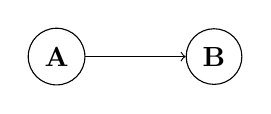
\begin{tikzpicture}[node distance=2cm]
        \node[circle,draw] at (0,0) (A) {\bf A};
        \node[circle,draw,right of=A] (B) {\bf B};
        \draw[->] (A) -- (B);
        \end{tikzpicture}
        \caption{Direct causality}
        \label{fig:direct_causation}
    \end{subfigure}
    \hfill
    \begin{subfigure}[b]{0.3\textwidth}
        \centering
        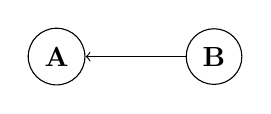
\begin{tikzpicture}[node distance=2cm]
        \node[circle,draw] at (0,0) (A) {\bf A};
        \node[circle,draw,right of=A] (B) {\bf B};
        \draw[<-] (A) -- (B);
        \end{tikzpicture}
        \caption{Reversed causality}
        \label{fig:reversed_causation}
    \end{subfigure}
    \hfill
    \begin{subfigure}[b]{0.3\textwidth}
        \centering
        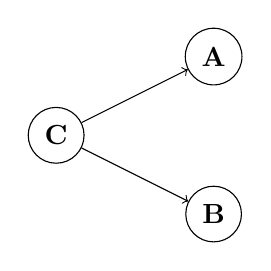
\begin{tikzpicture}[node distance=2cm]
        \node[circle,draw] at (0,0) (C) {\bf C};
        \node[circle,draw,right of=C,yshift=1cm] (A) {\bf A};
        \node[circle,draw,right of=C,yshift=-1cm] (B) {\bf B};
        \draw[->] (C) -- (A);
        \draw[->] (C) -- (B);
        \end{tikzpicture}
        \caption{Common causality}
        \label{fig:common_causation}
    \end{subfigure}
    \caption{Causality}
    \label{fig:causal_relationships}
    
\end{figure}

%\subsection{Case study}
Determining the causality from real world data is a difficult yet important task. Proving that the emission of green house gases causes global warming, is perhaps the most important task of our time? A more modest task is however addressed in this paper: investigating a possible causal relationship between thrust allocation and fuel consumption of a double ended ferry -- Uraniborg (\autoref{fig:uraniborg}).  
\begin{figure}[!htb]
    \centering
    \includegraphics[width=0.7\textwidth]{figures/GA_uraniborg.pdf}
    \caption{Double ended ferry Uraniborg, copyright Rederi AB Ventrafiken.}
    \label{fig:uraniborg}
\end{figure}
The thrust allocation concerns the load balance between the the ship's two azimuth thrusters: one in the aft, and one in the bow of the ship (\autoref{fig:uraniborg}). The two thrusters can run simultaneously, adding up to the total thrust force, driving the ship forward. The load balance can vary between all combinations from: full aft, to full forward thruster utilization. This balance can be expressed with $\alpha_{aft}$ as defined in \autoref{eq:aft_thrust_ratio},  
\begin{equation}
    \alpha_{aft} = \frac{C_{aft}}{C_{aft} + C_{fwd}}
    \label{eq:aft_thrust_ratio}
\end{equation}
where $C_{aft}$ and $C_{fwd}$ are the fuel consumption from the aft and forward thruster. 
\autoref{fig:fuel_consumption_correlation} shows data from trips between Landskrona and Ven during one year for the variables: total fuel consumption, and $\alpha_{aft}$. There seems to be a clear correlation between these variables,  which implies that there is relationship between them. But is it a direct causal relationship? Direct causality would mean that $\alpha_{aft}$ can be used as an optimization parameter to reduce the fuel consumption.
\begin{figure}[!htb]
    \centering
    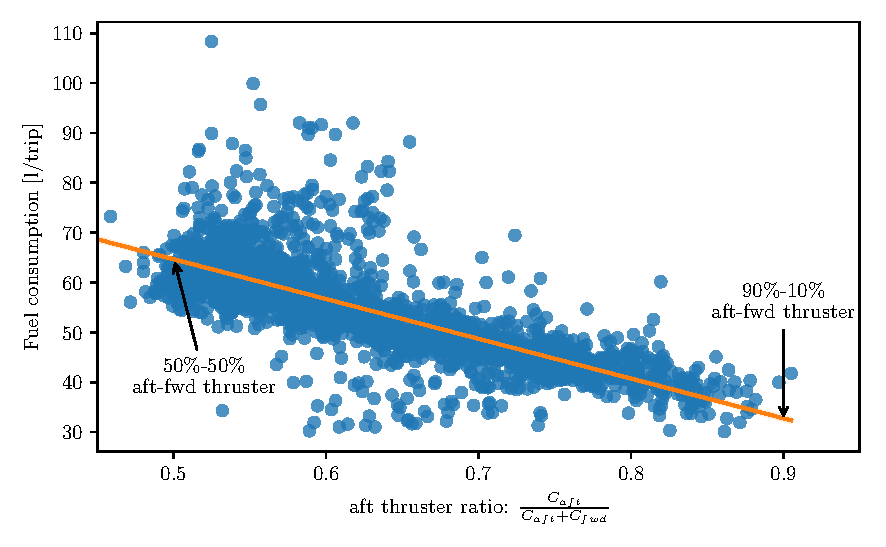
\includegraphics[width=\textwidth]{figures/correlation.pdf}
    \caption{Fuel consumption per trip with Uraniborg for trips during one year with varying aft thrust ratio.}
    \label{fig:fuel_consumption_correlation}
\end{figure}
%________________________________________
%Problem:
However, both reversed causality or common causality are other possibilities, considering for instance these hypothetical scenarios:
\begin{itemize}
    \item Increased fuel consumption forces a reduced aft thruster utilization if the aft thruster is not strong enough. The forward thruster is then needed to add up to the higher power demand. (Reversed causality)
    
    \item There is a hidden variable such as bad weather which forces both thrusters to be used. (Common causality)
\end{itemize}
%________________________________________

%Solution/Evaluation:
A blinded experiment was conducted onboard Uraniborg to infer the direct causal relationship. Results from this experiment are presented and analyzed in this paper to conclude the relationship. Alternative methods applicable when experiments are not possible, are also discussed and investigated. Conducting system identification on a well established physical model is one of these methods, which is presented in this paper. Also Monte Carlo simulations, and Markov chain analysis are alternatives that are discussed, but more briefly. To complete this paper, it is investigated if the alternative methods can reach to the same conclusion as obtained from the blinded experiment inference. 

\section{Method}
A blinded experiment (\autoref{sec:blinded_experiment}) is the classic way to determine the causation. For situations where experiments cannot be conducted system identification with well established
mathematical models, Monte Carlo simulations and Markov chain analysis are other methods.

\subsection{Blinded experiment}\label{sec:blinded_experiment}
In the blinded experiment, every other trip with Uraniborg was run with two different crews. One crew was operating as normal and the other crew was instructed to only use the aft thruster as much as possible. The same correlation that was seen in \autoref{fig:fuel_consumption_correlation} was observed again during the experiment and a direct causation was concluded that a higher use of the aft thruster will reduce the fuel consumption.

\subsection{System identification}
\subsection{Monte Carlo simulations}
\subsection{Markov chain analysis}

\section{Results}


The fuel consumption of Uraniborg with the speed correction applied, is shown in \autoref{tab:means_corrected} for the four datasets: ship operation by the captain and mate during experiment and the reference period. The captain had much lower fuel consumption compared to the mate for both periods. Even though the captain used a little bit higher aft thruster utilization already before the experiment (0.8 compared to 0.7), there can also be other explanations to the captains's lower consumption such as: higher skills and experience in operating the ship. 
The difference was however much larger during the experiment (\savingpctexperiment \%), compared to the reference period ({glue:}`saving_pct_before_experiment` %). The captain used a lower aft thruster utilization (TU=0.8) before the experiment compared to during the experiment, where aft thruster was used exclusively (TU=1). This means that at least {glue:}`saving_thruster_allocation_pct` % of the total {glue:}`saving_pct_experiment` % reduction can be accounted to the increased aft thruster utilization. 
The remaining difference between the fuel consumption of the captain and mate during the experiment ({glue:}`saving_pct_before_experiment` %) needs futher investigations. It would be a good idea to get a closer look at how the captain and mate operate the ship, to find an explanation how to operate the ship in the more energy efficient way of the captain.

\begin{table}[h]
    \centering
    \caption{Mean values corrected for differences in speed in the original data for the four datasets where the ship is operated by the captain or mate during the reference period or experiment.}
    \label{tab:means_corrected}
    \pgfplotstabletypeset[col sep=comma,
    columns={Operator,Period, sog, TU,Consumption,Trips},
    columns/Operator/.style={string type},
    columns/Period/.style={string type},
    column type=l,	% specify the align method
	every head row/.style={before row=\hline,after row=\hline},	% style the first row
	every last row/.style={after row=\hline},	% style the last row
	%every first column/.style={column type/.add={|}{}},	% style the first column
	%every last column/.style={column type/.add={}{|}},	% style the last column
    ]{tables/tab_means_corrected.csv}
\end{table}

\bibliography{sample}

\end{document}